\chapter{Lichtablenkung an einem Galaxiencluster\label{chapter:cluster}}
\lhead{Lichtablenkung an einem Galaxiencluster}
\begin{refsection}
\chapterauthor{Pascal Stump}

\section{Einleitung}
\rhead{Einleitung}
Wenn ein sehr massereiches Objekt zwischen einem Betrachter und einer
Lichtquelle platziert ist, tritt ein Gravitationslinseneffekt auf.  In
\index{Gravitationslinse}%
der Abbildung \ref{fig:lrg3-757} sieht man ein Beispiel, bei welchem
die Vordergrund-Galaxie (gelb/orange) praktisch in einer Linie zur
Hintergrund-Galaxie (blau) steht.  Durch die beinahe optimale
Ausrichtung in einer Linie wird die Hintergrund-Galaxie zu einem
Kreis verzerrt.  Der dabei entstehende Kreis wird auch Einsteinring
\index{Einsteinring}%
genannt.

Wenn die Vordergrund-Galaxie nicht rotationssymmetrisch ist, kann die
Hintergrund-Galaxie zu einzelnen Punkten verzerrt werden, so zu sehen
in der Abbildung \ref{fig:einsteinkreuz}.  Dabei ist die
Vordergrund-Galaxie wieder in der Mitte zu finden und die vier
umliegenden Punkte sind die verzerrte Hintergrund-Galaxie.

Ein drittes Beispiel des Gravitationslinseneffekts ist in Abbildung
\ref{fig:abell} zu finden.  Dabei ist nicht nur eine Galaxie als Linse
zuständig, sondern ein Galaxiencluster.  Die Vordergrund-Galaxien ist
wiederum die gelb, orange farbigen Galaxien.  Man sieht schön, dass
die Hintergrund-Galaxien zu Streifen verzogen werden und nicht mehr zu
einem ganzen Kreis, da die Ausrichtungen zueinander nicht optimal
sind.

\begin{figure}
  \centering
  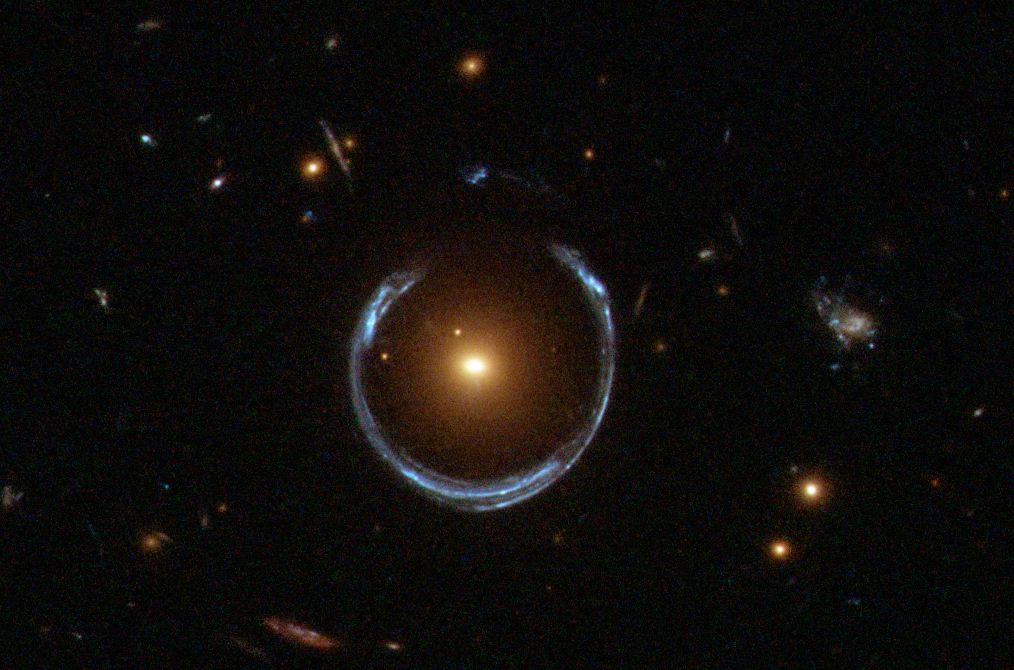
\includegraphics[width=\textwidth]{cluster/images/LRG_3-757}
  \caption{Einsteinring (LRG 3-757; ESA/Hubble \& NASA)
    \cite{nasa:einsteinring, wiki:einsteinring}}
  \label{fig:lrg3-757}
\end{figure}

\begin{figure}
  \centering
  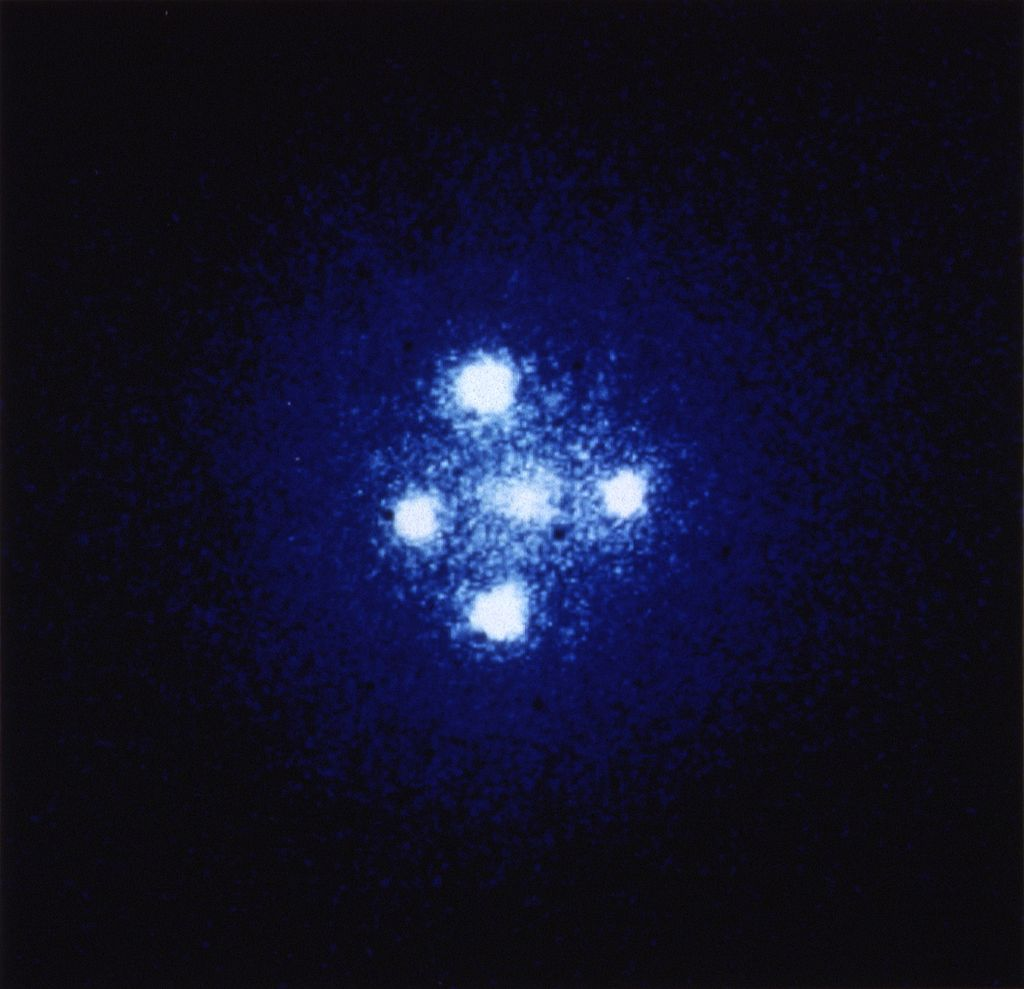
\includegraphics[width=.7\textwidth]{cluster/images/Einstein_cross}
  \caption{Einsteinkreuz (G2237+0305; NASA, ESA \& STScl)
    \cite{wiki:einsteinkreuz}}
  \label{fig:einsteinkreuz}
\end{figure}

\begin{figure}
  \centering
  \includegraphics[width=\textwidth]{cluster/images/HSTCI_PR00-08}
  \caption{Galaxiencluster (Abell 2218; NASA, ERO Team)
    \cite{wiki:abell}}
  \label{fig:abell}
\end{figure}

\section{``Normale'' Linse}
\rhead{Normale Linse}
Zuerst einmal ein Rückblick wie eine ``normale'' Linse funktioniert.
Eine ``normale'' Linse nutzt die Brechung zwischen dem Linsenmaterial
und seiner Umgebung aus.  Durch diese Brechung kommt es zu einer
Winkeländerung des Lichtstrahls.  Bei homogenen Materialien mit
bekannten Brechungsindizes kann folgende Formel aus der geometrischen
Optik verwendet werden:

\begin{equation}
  \frac{\sin \varepsilon_1}{\sin \varepsilon_2} = \frac{n_2}{n_1}.
\end{equation}

Darin kommen die Winkel zur Oberflächennormalen im Sinus-Bruch
und die beiden Brechungsindizes vor.  Der
Brechungsindex eines Mediums \(n\), ergibt sich aus der
Lichtgeschwindigkeit im Vakuum \(c\) geteilt durch die
Lichtgeschwindigkeit \(u\) im Medium:

\begin{equation}
  n = \frac{c}{u}.
\end{equation}
\index{Brechungsindex}


\subsection{Prinzip von Huygens}
\rhead{Prinzip von Huygens}
\index{Huygens!Prinzip von}%
\index{Prinzip von Huygens}%
Wie sich das Licht ausbreitet lässt sich anschaulich mit dem Prinzip
von Huygens aufzeigen.  In der Abbildung \ref{fig:huygens1} ist die
Lichtwellenausbreitung in einem homogenen Medium gezeigt.  Die
Lichtwelle (rote Linie unten) ist nach einem Zeitschritt
(\(\Delta t\)) an der mittleren Position zu finden.  Nach einem
weiteren \(\Delta t\) ist die Lichtwelle an der Position der obersten
roten Linie.  In der Abbildung bewegt sich die Lichtwelle von unten
nach oben.  Weil es sich um ein homogenes Material handelt, sind die
Abstände zwischen den Lichtwellen parallel und immer im gleichen
Abstand.  Das Prinzip von Huygens sagt nun, dass man von jedem Punkt
aus auf einer Lichtwelle (rote Linie), einen Halbkreis in
Ausbreitungsrichtung einzeichnen kann.  Der Halbkreis ist die Distanz,
welche das Licht nach \(\Delta t\) zurückgelegt hat.  Legt man nun
eine Umhüllende um die Halbkreise, erhält man die Position der
Lichtwelle zum neuen Zeitpunkt.

\begin{figure}
  \centering
  %
% Brechung nach dem Prinzip von Huygens


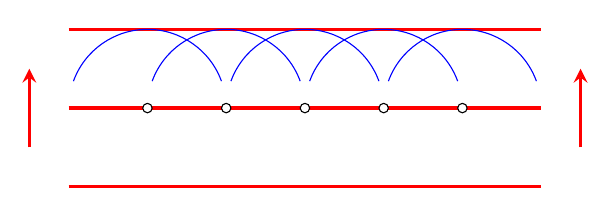
\begin{tikzpicture}

  
  % Delta t
  \foreach \y in {-1,0,1}
    \draw [very thick, color=red] (0,\y) -- (6,\y);

  \foreach \x in {1,2,3,4,5}
    \draw [black, fill=white] (\x,0) circle (.6mm);

  \foreach \x in {1,2,3,4,5}
    \draw [blue] (\x,0) ++ (0,1) arc (90:160:1cm)
                 (\x,0) ++ (0,1) arc (90:20:1cm);

  \draw [very thick, color=red, ->, >=stealth] (-.5,-.5) -- (-.5,0.5);
  \draw [very thick, color=red, ->, >=stealth] (6.5,-.5) -- (6.5,0.5);


\end{tikzpicture}
  \caption{Lichtwellen Ausbreitung nach dem Prinzip von Huygens.}
  \label{fig:huygens1}
\end{figure}

Hat man zwei verschiedenen homogene Materialien, kommt es zur
Brechung, welche auch mit dem Prinzip von Huygens gezeigt werden kann.
In der Abbildung \ref{fig:huygens2} kommt die Lichtwelle von oben
links.  Zum Zeitpunkt in dem die Lichtwelle die beiden Punkte \(A\)
und \(B\) bildet, berührt die Lichtwelle im Punkt \(A\) den
Materialübergang.  Zeichnet man nun die ``Bewegungs-Halbkreise'' ein,
so ist der Halbkreis ausgehend von \(B\) grösser als von \(A\).  Der
Grund dafür ist die höhere Lichtgeschwindigkeit im weissen Medium als
im blauen Medium.  Legt man von \(D\) aus die Tangente an den von
\(A\) ausgehenden Halbkreis, erhält man die Lichtwelle nach
\(\Delta t\).  Es ist gut sichtbar, dass die Lichtwelle
\(\overline{CD}\) gebrochen wurde und nicht parallel zu
\(\overline{AB}\) liegt.

\begin{figure}
  \centering
  %
% Brechung nach dem Prinzip von Huygens


\begin{tikzpicture}
  [every label/.style={color=black}]

  
  % Oberfläche
  \fill [fill=blue!15!white] (0,0) rectangle (6,-2);
  \draw [thick] (0,0) -- (6,0);
  \coordinate[label=below left:$A$] (A) at (3,0);
  \path (A) ++ (2,0) coordinate[label=below right:$D$] (D);

  \draw [very thick, color=red, -<, >=stealth] (A) --++ (150:2.5) node(ray1Start){};
  \path [name path=rayStart] (ray1Start.center) --++ (60:2.5);
  \path [name path=ray2] (A) ++ (2,0) --++ (150:6);
  \draw [very thick, color=red, name intersections={of=rayStart and ray2,
    by=ray2Start}, -<, >=stealth] (A) ++ (2,0) -- (ray2Start);

  \path (ray2Start) ++ (-30:2.5) coordinate[label=above:$B$] (B);
  \draw [color=red] (A) -- (B);


  \draw [thick, color=blue] (A) ++ (.8,0) arc (0:-180:.8cm);
  \draw [thick, color=blue]
    let \p1 = ($(B)-(D)$)
    in (B) ++ (-30:{veclen(\x1,\y1)}) arc (-30:140:{veclen(\x1,\y1)})
       (B) ++ (150:{veclen(\x1,\y1)}) coordinate (Bs)
       (A) ++ (150:{veclen(\x1,\y1)}) coordinate (As);

  \draw [color=red] (As) -- (Bs);

  \node [circle] (circleSmall) at (A) [minimum size=2*.8cm,
    inner sep=0]{};
  \draw [color=red] (D) -- (tangent cs:node=circleSmall, point={(D)},
    solution=2) coordinate[label=below left:$C$] (C);


  \path (C) ++ ($ (C)-(A) $) coordinate (Cs);
  \path (D) ++ ($ (C)-(A) $) coordinate (Ds);
  \draw [very thick, color=red, ->, >=stealth] (A) -- (C) -- ($ (C)!1.4!(Cs) $);
  \draw [very thick, color=red, ->, >=stealth] (D) -- ($ (D)!1.4!(Ds) $);
  \draw [color=red] (Cs) -- (Ds);

  \foreach \point in {A,B,C,D}
    \draw [black, fill=white] (\point) circle (.6mm);


\end{tikzpicture}
  \caption{Brechung nach dem Prinzip von Huygens.}
  \label{fig:huygens2}
\end{figure}

Im Fall der Gravitationslinse gibt es im Weltall natürlich keine starr
begrenzte homogene Bereiche.  Besser zum Vergleich geeignet ist die
Abbildung \ref{fig:huygens3} mit einem inhomogenen Material.  Durch
die tiefere Lichtgeschwindigkeit im blauen Material ist der Abstand
zwischen den Lichtwellen kleiner als im weissen Material, somit biegt
sich der Lichtstrahl.

Da die Lichtgeschwindigkeit in einem Gebiet mit hoher Gravitation
langsamer vergeht, biegen sich Lichtstrahlen in Richtung massen
schwere Objekte.  (Zum Beispiel könnte im Zentrum der blauen Fläche
ein Stern stehen.  Licht, welches nahe dem Stern vorbeigeht, wird in
Richtung des Sterns abgelenkt.)

\begin{figure}
  \centering
  %
% Brechung nach dem Prinzip von Huygens


\begin{tikzpicture}
  [every label/.style={color=black}]

  
  %

  \shade [inner color=blue!50!white, outer color=white] (-.6,0.55) circle (1.5cm);

  \coordinate (A) at (0,0);
  \coordinate (B) at (3,0);
  \draw [very thick, color=red] (A) -- (B);

  \path (B) ++ (97:1cm) coordinate (Bs);
  \path (Bs) ++ ($ (A)!1!187:(B) $) coordinate (As);
  \draw [very thick, color=red] (As) -- (Bs);

  \path (Bs) ++ (104:1cm) coordinate (Bss);
  \path (Bss) ++ ($ (A)!1!194:(B) $) coordinate (Ass);
  \draw [very thick, color=red] (Ass) -- (Bss);

  \draw [very thick, color=red] (A) ++ (0,-1) --++ ($ (B)-(A) $);
  \draw [very thick, color=red] (Bss) ++ (104:1cm) --++ ($ (A)!1!194:(B) $);

  
  % \fill [fill=blue!15!white] (0,0) rectangle (6,-2);
  % \draw [thick] (0,0) -- (6,0);
  % \coordinate[label=below left:$A$] (A) at (3,0);
  % \path (A) ++ (2,0) coordinate[label=below right:$D$] (D);

  % \draw [very thick, color=red, -<, >=stealth] (A) --++ (150:2.5) node(ray1Start){};
  % \path [name path=rayStart] (ray1Start.center) --++ (60:2.5);
  % \path [name path=ray2] (A) ++ (2,0) --++ (150:6);
  % \draw [very thick, color=red, name intersections={of=rayStart and ray2,
  %   by=ray2Start}, -<, >=stealth] (A) ++ (2,0) -- (ray2Start);

  % \path (ray2Start) ++ (-30:2.5) coordinate[label=above:$B$] (B);
  % \draw [color=red] (A) -- (B);


  % \draw [thick, color=blue] (A) ++ (.8,0) arc (0:-180:.8cm);
  % \draw [thick, color=blue]
  %   let \p1 = ($(B)-(D)$)
  %   in (B) ++ (-30:{veclen(\x1,\y1)}) arc (-30:140:{veclen(\x1,\y1)})
  %      (B) ++ (150:{veclen(\x1,\y1)}) coordinate (Bs)
  %      (A) ++ (150:{veclen(\x1,\y1)}) coordinate (As);

  % \draw [color=red] (As) -- (Bs);

  % \node [circle] (circleSmall) at (A) [minimum size=2*.8cm,
  %   inner sep=0]{};
  % \draw [color=red] (D) -- (tangent cs:node=circleSmall, point={(D)},
  %   solution=2) coordinate[label=below left:$C$] (C);


  % \path (C) ++ ($ (C)-(A) $) coordinate (Cs);
  % \path (D) ++ ($ (C)-(A) $) coordinate (Ds);
  % \draw [very thick, color=red, ->, >=stealth] (A) -- (C) -- ($ (C)!1.4!(Cs) $);
  % \draw [very thick, color=red, ->, >=stealth] (D) -- ($ (D)!1.4!(Ds) $);
  % \draw [color=red] (Cs) -- (Ds);

  % \foreach \point in {A,B,C,D}
  %   \draw [black, fill=white] (\point) circle (.6mm);


\end{tikzpicture}
  \caption{Brechung nach dem Prinzip von Huygens in einem inhomogen
    Material.}
  \label{fig:huygens3}
\end{figure}


\section{Gravitationslinse}
\rhead{Gravitationslinse}
\subsection{Einfluss der Gravitation auf die Zeit}
\rhead{Einfluss der Gravitation auf die Zeit}
Als Start wird die Formel \eqref{skript:kruemmung:raumzeitabstand}
\begin{equation*}
  s^2 = -c^2 (t_1-t_2)^2 + (x_1-x_2)^2 + (y_1-y_2)^2 + (z_1-z_2)^2
\end{equation*}
aus dem Abschnitt über den Lichtkegel genommen.

Die Gravitationslinse beugt Lichtwellen, somit ist \(s^2=0\), da sich
die Wirkung mit Lichtgeschwindigkeit ausbreitet.  Wird zur
Vereinfachung \(c=1\) gesetzt, ergibt sich:
\begin{equation*}
  0 = -(t_1-t_2)^2 + (x_1-x_2)^2 + (y_1-y_2)^2 + (z_1-z_2)^2
\end{equation*}
oder anders geschrieben
\begin{equation*}
  0 = -dt^2 + dx^2 + dy^2 + dz^2.
\end{equation*}

Die Lichtwellen bewegen sich in minimalen Wegen, was den Geodäten
entspricht.  Die Lichtablenkung an Sternen und Galaxien befindet sich
im Bereich von schwachen Gravitationsfeldern.  Zu diesen wurden die
\(g_{\mu\nu}\):
\begin{align*}
  g_{00} &= -1 -\frac{2\varphi}{c^2} &g_{kk} &= 1,\quad k=1,2,3
\end{align*}
bereits berechnet (Formel \ref{skript:gravitation:naeherung}).
Das Gravitationspotential \(\varphi\) ist für eine Punktmasse:
\begin{equation*}
  \varphi = -\frac{KM}{r}
\end{equation*}
\(M\) ist die Punktmasse, \(K\) die Gravitationskonstante
(oft als \(G\) bezeichnet) und \(r\) der Abstand zur Punktmasse.
Setzt man dies nun zusammen, erhält man folgende \(g_{\mu\nu}\):
\begin{align*}
  g_{00} &= -1 +\frac{2KM}{rc^2} &g_{kk} &= 1,\quad k=1,2,3.
\end{align*}
Für grosse Abstände \(r\) wird \(g_{00}=-1\).  Was gleich der normalen
Minkowski-Metrik ist.

\begin{beispiel}
  In folgendem soll die Zeitveränderung für Werte unserer Sonne
  berechnet werden.  Die Werte sind:
  \begin{align*}
    K &= \SI{6.67e-11}{\meter\cubed\per\kilogram\per\second\squared}
    &M &= \SI{1.99e30}{\kilogram}
    &c &= \SI{2.99e8}{\meter\per\second}.
  \end{align*}
  Die Zeitveränderung wird nur vom zweiten Teil von \(g_{00}\)
  bestimmt, wobei man erhält:
  \begin{align*}
    \tilde{t} &= \frac{2KM}{rc^2}
    &\left[\tilde{t}\right] &=
                              \si{\meter\cubed\per\kilogram\per\second\squared}
                              \cdot \si{\kilogram}
                              \cdot \si{\per\meter}
                              \cdot \si{\per\meter\squared\second\squared}
                              = 1.
  \end{align*}
  Einen Graphen mit den Werten von \(1\) bis \(0.05\) für
  \(\tilde{t}\) mit dem Abstand \(r\) kann in der Abbildung
  \ref{fig:bsp1} gefunden werden.  Ein \(\tilde{t}\) von \(0.25\)
  entspricht einer Verlangsamung von Wasser.  Je näher bei
  \(\tilde{t}=1\) desto langsamer bewegt sich das Licht, da
  \(g_{00} \rightarrow 0\) wird.  Es ist zu beachten, dass das
  geplotete maximale \(r\) von \SI{60000}{\meter} immer noch innerhalb
  der Sonne ist, da der Sonnenradius \SI{\approx\, 700e6}{\meter}
  entspricht.
  \begin{figure}
    \centering
    

\begin{tikzpicture}[scale = 1.7]
    \datavisualization[scientific axes = clean,
                     y axis = {grid,
                               label=\(\tilde{t}\) von \(1\) bis \(0.05\),
                               min value = 0,
                               max value = 1},
                     x axis = {grid,
                               label=\(r\) in \si{\meter},
                               min value = 0,
                               max value = 60000},
                     visualize as smooth line/.list={ch1},
                     style sheet=vary hue,
                     %style sheet=vary dashing,
                     %ch1={label in legend={text=Mittenkavität}},
                     ]
                    
  data [set=ch1,headline={x, y}, read from file=cluster/source/bsp1.csv];
\end{tikzpicture}
    \caption{\(\tilde{t}\) von \(1\) bis \(0.05\)}
    \label{fig:bsp1}
  \end{figure}
\end{beispiel}

Im obigen Beispiel ist gut ersichtlich, wie schnell der Einfluss der
Gravitation abnimmt.  Eine Linse mit dieser Eigenschaft müsse so
geformt sein, wie ein Weinglasboden.  In der Abbildung
\ref{fig:ModelGravLinse} sind drei Beispielkonstellationen zu sehen.
Ist der Weinglasboden in einer Linie mit der Kerze (unten links)
erhält man ein Einsteinring ähnliches Gebilde.  Bei einem gekippten
Boden (oben rechts) erhält man beinahe ein Einsteinkreuz.  Und unten
\index{Einsteinkreuz}%
rechts sieht man ein Beispiel was passiert, wenn die Linse und die
Quelle nicht in einer Linie stehen (wie im Cluster Bild
\ref{fig:abell}).

\begin{figure}
  \centering
  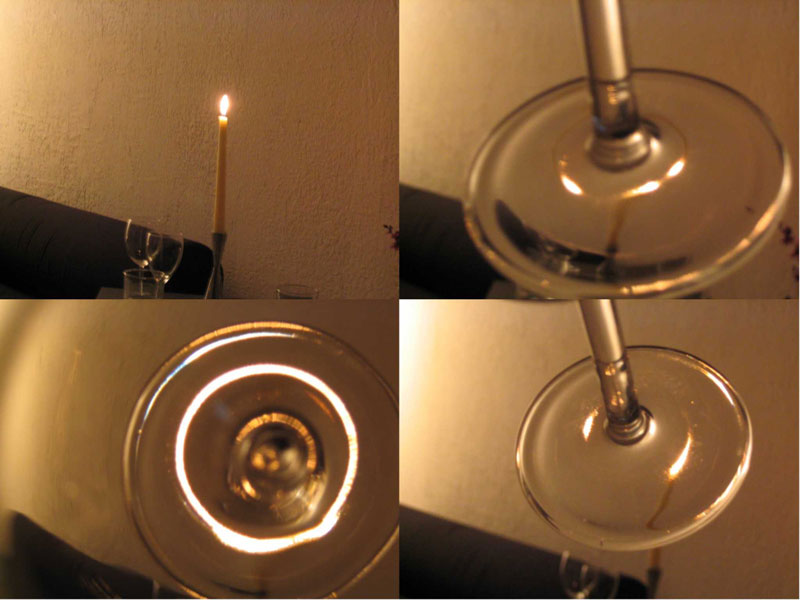
\includegraphics[width=\textwidth]{cluster/images/model_grav_lens}
  \caption{Model einer Gravitationslinse (Boden eines Weinglases)
    \cite{standford:ModelGravLens}}
  \label{fig:ModelGravLinse}
\end{figure}

\subsection{Euler-Lagrange}
\rhead{Euler-Lagrange}
\index{Euler-Lagrange-Gleichungen}%
Um die Lichtablenkung zu berechnen, benötigt man den Weg des Lichts
\index{Lichtablenkung}%
und nicht nur wie stark die Lichtgeschwindigkeit abgebremst wird.  Das
Licht nimmt den Weg mit der kürzesten Laufzeit.  Aus der Physik kennt
man, dass die Zeit gleich der Strecke durch die Geschwindigkeit ist:
\begin{equation*}
  t = \frac{s}{v}.
\end{equation*}

Für den Weg des Lichts muss man somit jedes Wegstück mit seiner
Geschwindigkeit dividieren und all diese Stückchen zusammen addieren.
Das Licht nimmt nun den Weg, in welchem es die kürzeste Laufzeit hat.
Um eine Strecke zu minimieren, kann man Euler-Lagrange verwenden,
welche ein Integral der Form
\begin{equation*}
  I = \int\limits_{t_0}^{t_1}\! F\bigl(x^{\alpha}(t), \dot{x}^{\alpha}(t),t\bigr)d t
\end{equation*}
benötigt.  Das Integral soll die Zeit minimieren, somit muss es einen
Weg geteilt durch eine Geschwindigkeit im Integral geben.  Eine
Möglichkeit ist folgendes Integral:
\begin{equation}
  I = \int\! \sqrt{\dot{x}(l)^2+\dot{y}(l)^2+\dot{z}(l)^2} \cdot
  \frac{n\bigl(x(l),y(l),z(l)\bigr)}{c} d l.
\end{equation}

Der Wert unter der Wurzel entspricht dem Wegstück während eines
Integrationsschritts.  Die Division entspricht eins durch die
Geschwindigkeit.  Somit erhält man im Integral eine Zeit, welche über
den gesamten Weg integriert der Wegzeit des Lichts entspricht.  Da die
Lichtgeschwindigkeit \(c\) unabhängig von der Position ist, kann man
den Bruch vor das Integral nehmen:
\begin{equation}
  I = \frac{1}{c}\int\! \sqrt{\dot{x}(l)^2+\dot{y}(l)^2+\dot{z}(l)^2}
  \cdot n\bigl(x(l),y(l),z(l)\bigr) d l.
\end{equation}
Des Weiteren benötigt man für Euler-Lagrange nur den Teil im Integral:
\begin{equation}
  L = \sqrt{\dot{x}(l)^2+\dot{y}(l)^2+\dot{z}(l)^2}
  \cdot n\bigl(x(l),y(l),z(l)\bigr).
\end{equation}
Da die Wurzel die folgenden Rechenschritte verkompliziert, wird sie
quadriert, was das Extremum nicht verändert.  Dieser Schritt wurde
bereits im Abschnitt
\ref{skript:geodaeten:subsection:Parametrisierung} angewendet.  Weiter
wird die Abhängigkeit von \(l\) nicht mehr geschrieben, was es
natürlich bleibt:
\begin{equation}
  F = L^2 = (\dot{x}^2+\dot{y}^2+\dot{z}^2)n^2.
\end{equation}

Für Euler-Lagrange muss man nun dieses \(F\) ableiten, im folgenden
nur mit \(x\) gezeigt:
\begin{equation}
  \label{eq:cluster:euler}
  0 = \frac{\partial F}{\partial x} - \frac{d}{d l} \frac{\partial
    F}{\partial \dot{x}}.
\end{equation}
Die Ableitungen sind
\begin{align*}
  \frac{\partial F}{\partial x} &= (\dot{x}^2+\dot{y}^2+\dot{z}^2) 2n
                                  \frac{\partial n}{\partial x}\\
  \frac{\partial F}{\partial\dot{x}} &= 2\dot{x}n^2\\
  \frac{d}{d l}\frac{\partial F}{\partial\dot{x}} &= 2\ddot{x}n^2 + 4\dot{x}n
                                \left(\frac{\partial n}{\partial x}\dot{x} +
                                \frac{\partial n}{\partial y}\dot{y} +
                                \frac{\partial n}{\partial z}\dot{z} \right).
\end{align*}
Setzt man die obigen Berechnungen in \ref{eq:cluster:euler} ein und
löst diese Formel nach \(\ddot{x}\) auf, erhält man:
\begin{equation}
  \ddot{x} = (-\dot{x}^2+\dot{y}^2+\dot{z}^2)
  \frac{1}{n}\frac{\partial n}{\partial x} -
  2\dot{x}\dot{y} \frac{1}{n}\frac{\partial n}{\partial y} -
  2\dot{x}\dot{z} \frac{1}{n}\frac{\partial n}{\partial z}.
\end{equation}
Mit der Hilfe der logarithmischen Differentiation
\index{logarithmische Differentiation}%
\index{Differentiation, logarithmische}%
\begin{equation*}
  \frac{1}{n} \frac{\partial n}{\partial x} = \frac{\partial \ln
    n}{\partial x}
\end{equation*}
kann man die Formel weiter vereinfachen:
\begin{equation}
  \ddot{x} = (-\dot{x}^2+\dot{y}^2+\dot{z}^2) \frac{\partial \ln
    n}{\partial x} - 2\dot{x}\dot{y} \frac{\partial \ln n}{\partial y}
  - 2\dot{x}\dot{z} \frac{\partial \ln n}{\partial z}.
\end{equation}
Normalerweise ist ein Logarithmus nicht der einfachste Ansatz.  Die
Vereinfachung entsteht durch die spezielle Form von \(n\)
\begin{equation*}
  n \approx 1-\frac{2\varphi}{c^2}
\end{equation*}
und weil
\begin{equation*}
  \frac{\varphi}{c^2} \ll 1
\end{equation*}
ergibt sich
\begin{equation*}
  \ln n \approx -\frac{2\varphi}{c^2}.
\end{equation*}

Somit muss man nun keine partielle Ableitung von \(\ln n\), sondern von
\(-\frac{2\varphi}{c^2}\) durchführen (d.h. man braucht
\(\nabla\varphi=\) Gravitationskraft).  In einem Beispiel soll dies in
2D gezeigt werden.

\begin{beispiel}
  Im Folgenden wird die Lichtablenkung in einem zwei dimensionalen
  Raum numerisch berechnet.  Als \(\varphi\) wird eine Punktquelle
  verwendet:
  \begin{equation*}
    \varphi = -\frac{KM}{r}.
  \end{equation*}
  Wobei
  \begin{equation*}
    r = \sqrt{(x-x_L)^2+(y-y_L)^2}
  \end{equation*}
  der Abstand zwischen dem aktuellen Punkt und der Linse ist.

  Berechnet man mit Hilfe von Maxima Euler-Lagrange nach den beiden
\index{Maxima}%
  Koordinatenachsen, erhält man:
  \begin{align*}
    \ddot{x} &= -\frac{2(-\dot{x}^2+\dot{y}^2)(x-x_L)KM}
               {c^2\sqrt{(x-x_L)^2+y^2}\,^3}+
               \frac{4\dot{x}y\dot{y}KM}{c^2\sqrt{(x-x_L)^2+y^2}\,^3}\\
    \ddot{y} &= +\frac{4\dot{x}\dot{y}(x-x_L)KM}{c^2\sqrt{(x-x_L)^2+y^2}\,^3}
               - \frac{2(\dot{x}^2-\dot{y}^2)yKM}
               {c^2\sqrt{(x-x_L)^2+y^2}\,^3}.
  \end{align*}
  In diesem Beispiel befindet sich die Gravitationslinse auf \(x=0\),
  somit vereinfacht sich \(y-y_L\) zu \(y\).  Die soeben erhaltenen
  Formeln kann man in dieser Form noch nicht verwenden.  Man hat ein
  Differentialgleichungssystem zweiter Ordnung.  Was von geläufigen
  Computer Algorithmen nicht gelöst werden kann, da sie ein Differentialgleichungssystem
  erster Ordnung benötigen.

  Mit Substitution kann man eine Differentialgleichung zweiter Ordnung
  in ein Differentialgleichungssystem erster Ordnung überführen.  Macht man diese
  Substitution mit beiden Formeln, erhält man ein Gleichungssystem
  erster Ordnung, welche beide Formeln enthält.  Wählt man folgende
  Substitutionen
  \begin{align*}
    x_1 &= x &x_2 &= \dot{x} &x_3 &= y &x_4 &= \dot{y}
  \end{align*}
  kann man die beiden Formeln in eine brauchbare Form bringen.  Die
  gängigen Algorithmen fordern die Ableitungen von \(x_k\) als
  Parametern:
  \begin{align*}
    \dot{x}_1 &= x_2\\
    \dot{x}_2 &= -\frac{2\left(-x_2^2+x_4^2\right)\bigl(x_1-x_L\bigr)KM}
                {c^2\sqrt{\bigl(x_1-x_L\bigr)^2+x_3^2}\,^3}
                + \frac{4 x_2x_3x_4 KM}
                {c^2\sqrt{\bigl(x_1-x_L\bigr)^2+x_3^2}\,^3}\\
    \dot{x}_3 &= x_4\\
    \dot{x}_4 &= +\frac{4x_2x_4\bigl(x_1-x_L\bigr)KM}
                {c^2\sqrt{\bigl(x_1-x_L\bigr)^2+x_3^2}\,^3}
                - \frac{2 \left(x_2^2-x_4^2\right) x_3 KM}
                {c^2\sqrt{\bigl(x_1-x_L\bigr)^2+x_3^2}\,^3}.
  \end{align*}

  In Octave wird \(x_k\) zu \texttt{x(k)}, was zu folgendem Code
  führt:
  \lstinputlisting[style=Octave]{cluster/source/dglSubCode.m}

  Setzt Man nun die Werte
  \begin{align*}
    x_L &\approx \SI{150e6}{\kilo\meter} &M &\approx
                                              \SI{2e30}{\kilogram}
    &R &\approx \SI{700e3}{\kilo\meter}
  \end{align*}
  der Sonne ein,
  erhält man eine Winkeländerung von \(\approx \SI{1.75}{''}\),
  vergleicht man dies mit dem Wert aus der Literatur von
  \(\SI{1.75}{''}\) (\cite{misner1973gravitation} S.446), scheint
  dieses Vorgehen ziemlich adäquat.

  Im Graphen \ref{fig:lichtablenkungSonne} ist der numerisch
  berechnete Lichtweg dargestellt.  Der Beobachter ist im Punkt (0,0)
  und die Sonne im Punkt (\SI{1.5e11}{\meter},0).  Der Lichtpfad
  startet von der Erde aus so, dass man direkt am Sonnenradius
  vorbeischaut.  Da die Ablenkung nur \SI{1.75}{''} ist, sieht der Lichtweg
  von Auge betrachtet wie eine gerade Strecke aus.  (Eine Bogensekunde
  ist ein 3600stel eines Grades.)

  Nimmt man zur Berechnung eine schwerere Sonne an, ist die
  Lichtablenkung auch von Auge gut zu sehen.  In der Abbildung
  \ref{fig:lichtablenkung300Sonne} ist die Sonne 300 mal schwerer (bei
  gleichem Radius) und in \ref{fig:lichtablenkung600Sonne} sogar 600
  mal mehr.

  \begin{figure}
    \centering
    \begin{tikzpicture}[scale = 1.7]
      \datavisualization[scientific axes = clean,
                         y axis = {grid,
                                   label=\(y\) in \si{\meter},
                                   min value = 0,
                                   max value = 1.5e9},
                         x axis = {grid,
                                   label=\(x\) in \si{\meter},
                                   min value = 0,
                                   max value = 3e11},
                         visualize as smooth line/.list={ch1},
                         % ch1={style=very thick},
                         style sheet=vary hue,
                         % style sheet=vary dashing,
                         % ch1={label in legend={text=Mittenkavität}},
                        ]
                    
      data [set=ch1,headline={x, y}, read from file=cluster/source/lichtablenkungSonne.csv];
    \end{tikzpicture}
    \caption{Lichtablenkung an der Sonne}
    \label{fig:lichtablenkungSonne}
  \end{figure}
  
  \begin{figure}
    \centering
    \begin{tikzpicture}[scale = 1.7]
      \datavisualization[scientific axes = clean,
                         y axis = {grid,
                                   label=\(y\) in \si{\meter},
                                   min value = 0,
                                   max value = 1.5e9},
                         x axis = {grid,
                                   label=\(x\) in \si{\meter},
                                   min value = 0,
                                   max value = 3e11},
                         visualize as smooth line/.list={ch1},
                         % ch1={style=very thick},
                         style sheet=vary hue,
                         % style sheet=vary dashing,
                         % ch1={label in legend={text=Mittenkavität}},
                        ]
                    
      data [set=ch1,headline={x, y}, read from file=cluster/source/lichtablenkung300Sonne.csv];
    \end{tikzpicture}
    \caption{Lichtablenkung an 300 Sonnenmassen}
    \label{fig:lichtablenkung300Sonne}
  \end{figure}
  
  \begin{figure}
    \centering
    \begin{tikzpicture}[scale = 1.7]
      \datavisualization[scientific axes = clean,
                         y axis = {grid,
                                   label=\(y\) in \si{\meter},
                                   min value = 0,
                                   max value = 1.5e9},
                         x axis = {grid,
                                   label=\(x\) in \si{\meter},
                                   min value = 0,
                                   max value = 3e11},
                         visualize as smooth line/.list={ch1},
                         % ch1={style=very thick},
                         style sheet=vary hue,
                         % style sheet=vary dashing,
                         % ch1={label in legend={text=Mittenkavität}},
                        ]
                    
      data [set=ch1,headline={x, y}, read from file=cluster/source/lichtablenkung600Sonne.csv];
    \end{tikzpicture}
    \caption{Lichtablenkung an 600 Sonnenmassen}
    \label{fig:lichtablenkung600Sonne}
  \end{figure}
\end{beispiel}

Im vorherigen Beispiel sieht man gut, dass die Lichtstrahlen bis
praktisch zur Sonne eine Gerade darstellen, dann abgebogen werden und
wieder in einer Gerade weiterfliegen.  Stellt man nur diese Ablenkung
dar (\ref{fig:lichtablenkung600SonneZoom}) ist das noch besser
sichtbar.

\begin{figure}
  \centering
  \begin{tikzpicture}[scale = 1.7]
    \datavisualization[scientific axes = clean,
                       y axis = {grid,
                                 label=\(y\) in \si{\meter},
                                 min value = 6.5e8,
                                 max value = 7e8},
                       x axis = {grid,
                                 label=\(x\) in \si{\meter},
                                 min value = 1.4e11,
                                 max value = 1.6e11},
                       visualize as smooth line/.list={ch1},
                       % ch1={style=very thick},
                       style sheet=vary hue,
                       % style sheet=vary dashing,
                       % ch1={label in legend={text=Mittenkavität}},
                      ]
                    
    data [set=ch1,headline={x, y}, read from file=cluster/source/zoomLichtablenkung600Sonne.csv];
  \end{tikzpicture}
  \caption{Lichtablenkung an 600 Sonnenmassen (Zoom)}
  \label{fig:lichtablenkung600SonneZoom}
\end{figure}

Das Verhalten, dass über eine lange Strecke nichts passiert, erschwert
die nummerische Berechnung.  Die Algorithmen \texttt{ode23} und \texttt{ode45} in Octave
waren nicht in der Lage den Weg zu berechnen.  Hingegen konnte die
Lichtablenkung im Beispiel oben mit \texttt{ode23s} aus Octave berechnet
werden.  Dieser Algorithmus ist fähig steife Probleme zu berechnen.
Solche Probleme nennt man steif, wenn eine tiefe Frequenz von einer
hohen Frequenz überlagert wird.  Im weiteren Sinn ist dieses Problem
steif, da zwischen Beobachter, Gravitationslinse und Quelle sehr
grosse Abstände vorhanden sind, in denen nichts passiert.  Zum Lösen
berechnet \texttt{ode23s} auf der gesamten vorgegebenen Strecke Punkte.  Für
Sonnenabstände ist dies noch gut berechenbar, für Galaxienabstände
jedoch nicht.

\subsection{Bildverzerrung}
\rhead{Bildverzerrung}
Möchte man nun ein Bild der Lichtablenkung erzeugen, muss man für
jedes Pixel den Lichtweg simuliert.  Wenn man den einfachsten Fall der
Punktquelle beibehält, kann man die Symmetrie ausnützen und muss somit
nur ein Achtel der Pixelauflösung berechnen.

Für die Simulation wurde wieder der Abstand von der Erde zur Sonne
verwendet.  Um die Lichtablenkung noch zu verstärken, wurde die
tausendfache Sonnenmasse bei gleichem Radius angenommen.  Der
Pixelabstand in der Sonnenebene liegt bei \SI{10e6}{\meter}.  Das
Hintergrundbild, die Andromeda Galaxie aus Abbildung \ref{fig:m31},
ist in rund 6.8 fachem Sonnenabstand von der Erde aus platziert.  Der
Pixelabstand wurde gleich gewählt.

\begin{figure}
  \centering
  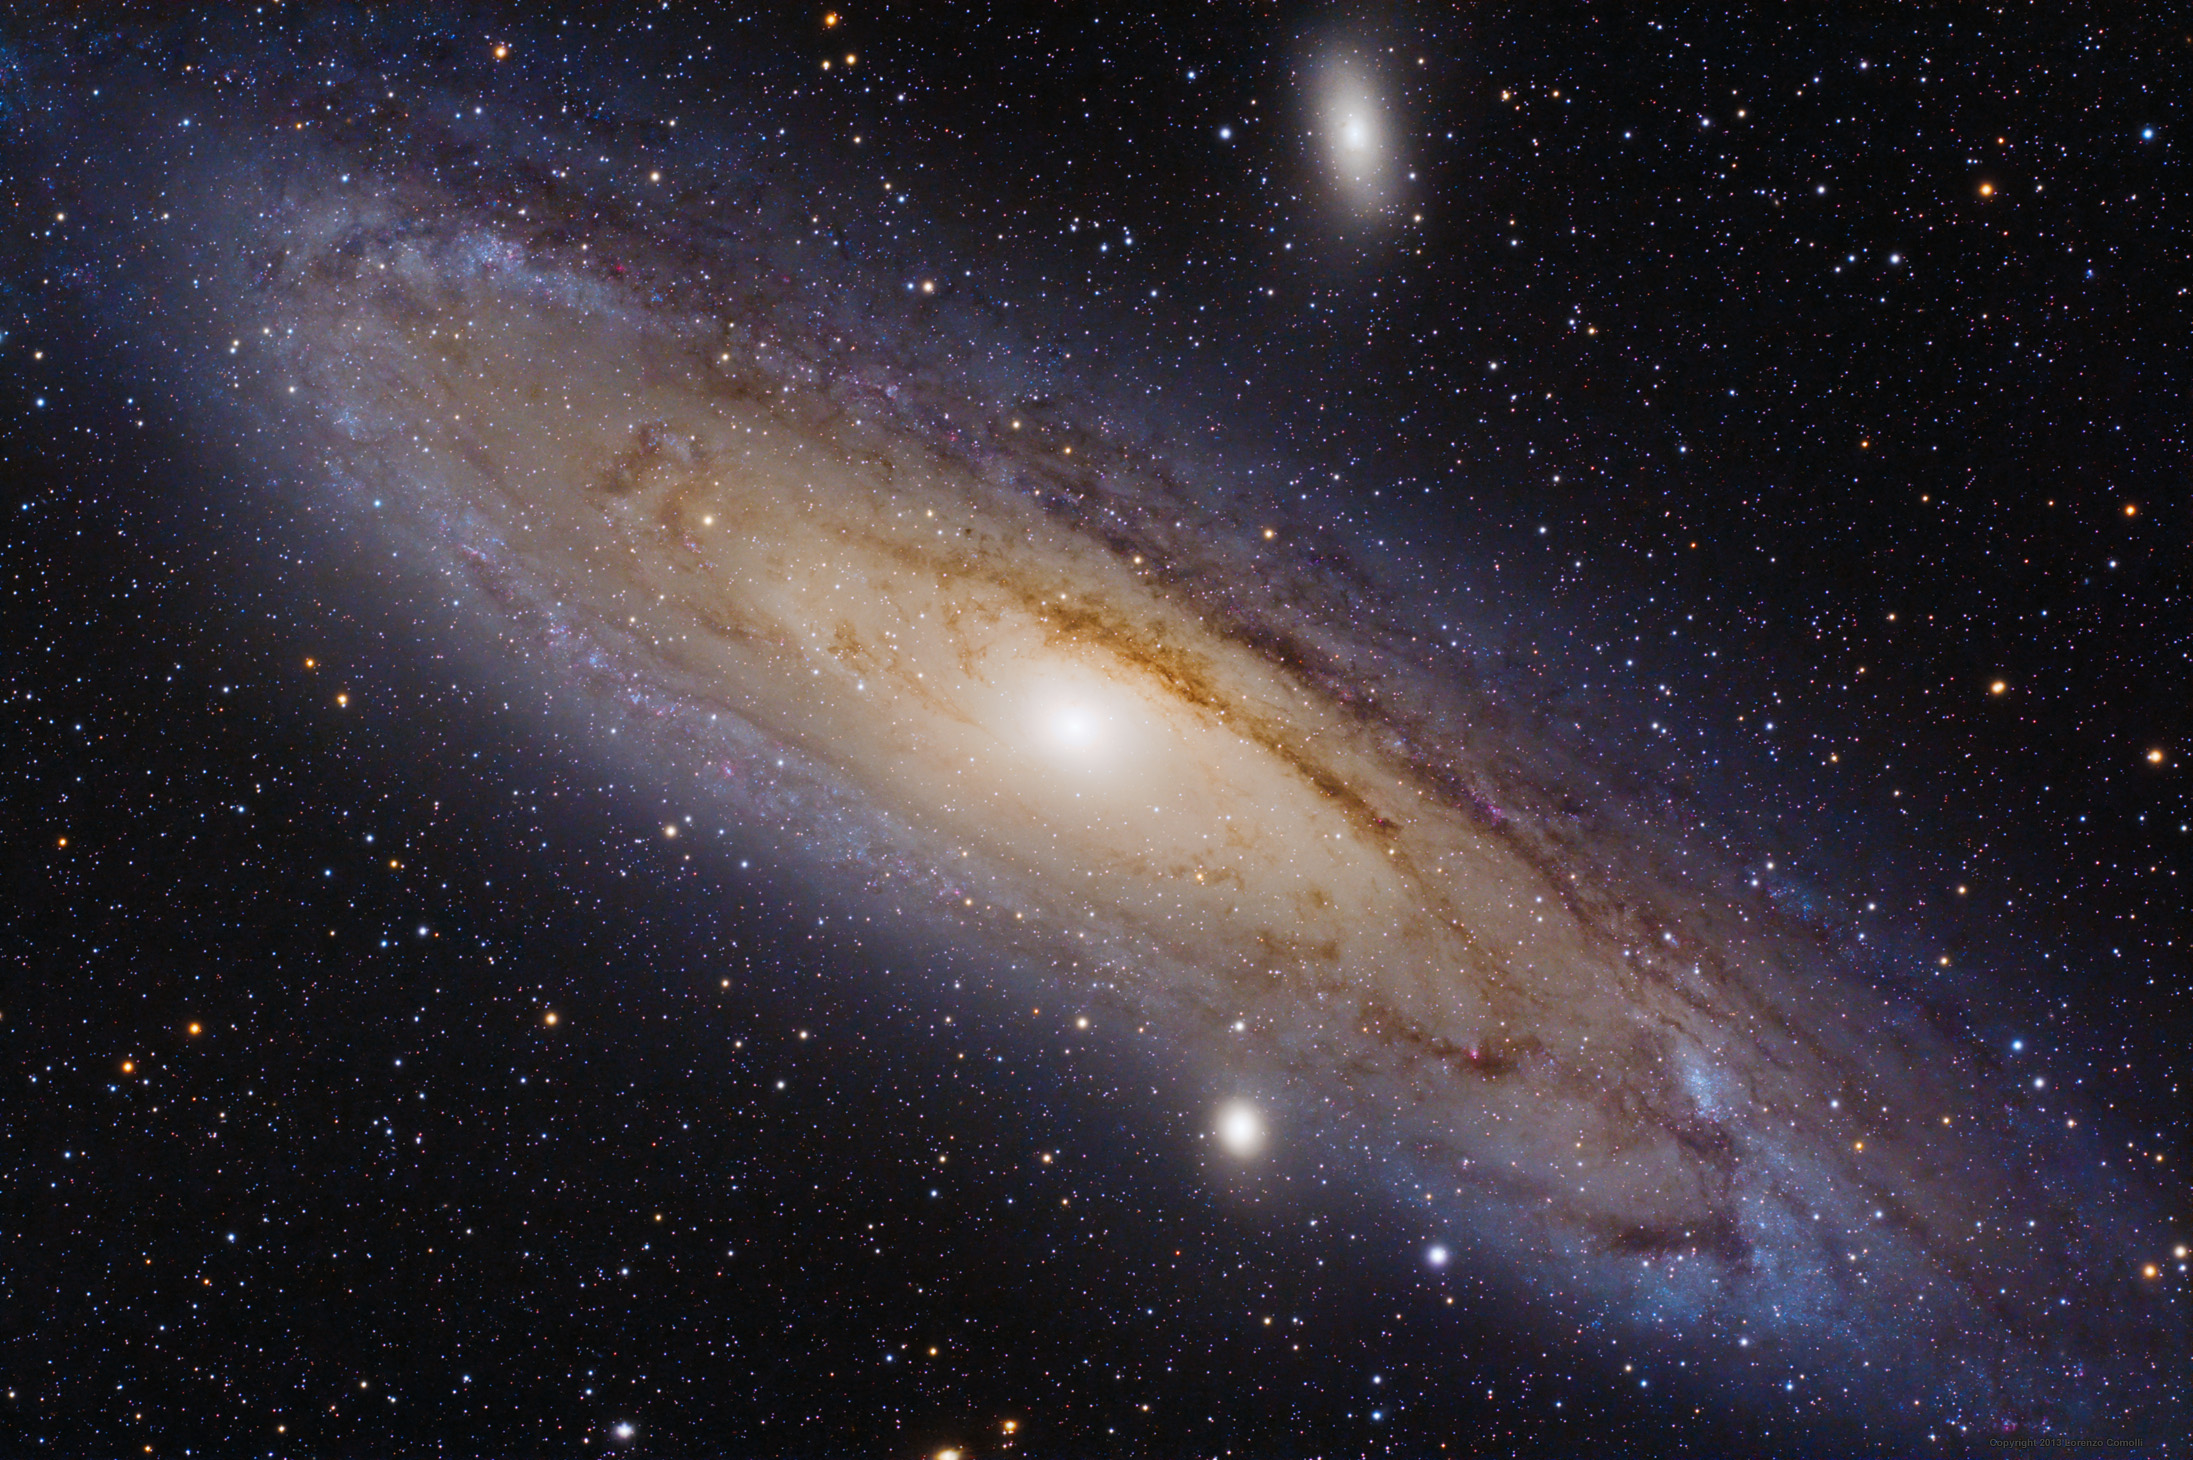
\includegraphics[width=\textwidth]{cluster/images/m31_comolli_2193}
  \caption{Andromeda Galaxie M31 \cite{nasa:andromedaM31}}
  \label{fig:m31}
\end{figure}

In der Abbildung \ref{fig:einsteinringSim} sieht man, wie das Zentrum
der Galaxie zu einem Ring verzogen wird.  Das schwarze Zentrum in der
Abbildung ist die Position der ``Sonne''.  Die Abbildung hat eine
Auflösung von \(300\times300\) Pixel und benötigte gut eineinhalb Tage
Berechnungszeit bei vier Kernen mit Hyper-Threading.

\begin{figure}
  \centering
  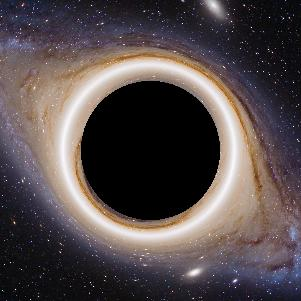
\includegraphics[width=.6\textwidth]{cluster/images/einsteinring}
  \caption{Bildverzerrung durch 1000 Sonnenmassen}
  \label{fig:einsteinringSim}
\end{figure}

\printbibliography[heading=subbibliography]
\end{refsection}

